\documentclass[12pt]{article}
\usepackage[a4paper,margin=25mm]{geometry}
\usepackage[T1]{fontenc}
\usepackage{mathptmx}
\usepackage{amsmath,amssymb}
\usepackage{booktabs,array,graphicx,xcolor,url}
\usepackage[super,comma,sort&compress]{natbib}
\usepackage{setspace}
\usepackage[modulo]{lineno}
\usepackage{tikz,pgfplots}
\usetikzlibrary{arrows.meta,positioning,fit}
\pgfplotsset{compat=1.17}
\usepackage[hidelinks]{hyperref}
\urlstyle{same}

% Nature: double-spaced text, line numbers, tables on their own pages,
% figure legends with their figures at initial submission.
\doublespacing
\linenumbers
\setlength{\parindent}{1.5em}
\setlength{\emergencystretch}{3em}
\renewcommand{\figurename}{Fig.}
\usepackage{caption}
\DeclareCaptionLabelSeparator{pipe}{ $\vert$ }
\captionsetup[figure]{labelsep=pipe, labelfont=bf, font=normalsize}
\captionsetup[table]{labelsep=pipe, labelfont=bf, textfont=bf, font=normalsize, justification=raggedright, singlelinecheck=false, skip=4pt}
\makeatletter
\renewcommand{\@biblabel}[1]{#1.}
\makeatother

\newcommand{\edtable}[3]{%
  \clearpage
  \noindent\textbf{Extended Data Table #1 \textbar{} #2}\par\smallskip
  {\singlespacing\footnotesize\noindent\input{generated/#3}\par}}

\begin{document}

\begin{flushleft}
{\Large\bfseries Authenticating the meaning of machine-generated text across languages\par}
\bigskip
Geunsik Lim\textsuperscript{1}\par
\medskip
{\small \textsuperscript{1}Independent researcher. Correspondence: leemgs@gmail.com\par}
\end{flushleft}

\bigskip

\noindent\textbf{%
Large language models now write fluent text at a scale that strains the information ecosystem, and regulators increasingly ask that synthetic content be marked in a machine-readable way\cite{euaiact2024}. Most text watermarks hide a statistical signal in the choice of individual words\cite{kirchenbauer2023kgw,dathathri2024synthid}, so translation or paraphrase, which replace those words while keeping the meaning, can remove the signal\cite{he2024crosslingual}. Semantic watermarks reduce this dependence on wording\cite{hou2024semstamp,liu2023sir}, but closeness in an embedding space cannot tell which particular fact, such as a negation, a quantity or a date, has changed. Here we show that provenance can instead be attached to the meaning itself. We represent each sentence as a typed record of the facts that must not change, register a keyed authentication tag over that record with the generating system, and verify a text by extracting the record again. On thousands of real machine translations, the record and its tag survive where a word-level watermark and similarity fingerprints do not, and a single altered fact is both rejected and located. The evidence comes from a closed, synthetic domain; it identifies open-vocabulary extraction of typed meaning as the capability that general-purpose provenance will need.}

\bigskip

Text produced by language models is increasingly reused, translated and rewritten before anyone asks where it came from. Knowing which text is synthetic also matters for training data, because models trained on unattributed synthetic text degrade over generations\cite{shumailov2024collapse}. Provenance signals are useful only if they survive ordinary transformations of the text\cite{liu2024survey}. Generation-time watermarks modify the sampling of each token so that an authorized detector can later find a statistical bias\cite{kirchenbauer2023kgw,dathathri2024synthid}; SynthID-Text showed that such a scheme can run in a production system without degrading quality\cite{dathathri2024synthid}. Because the signal lives in token choices, however, any transformation that replaces those choices while keeping the content, translation above all, can erase it\cite{he2024crosslingual}, and detector-guided paraphrasing can remove it deliberately\cite{cheng2025adversarial}. Other schemes add formal guarantees of robustness, freedom from distortion, undetectability, public verifiability or low false-positive rates\cite{zhao2023provable,kuditipudi2024distortionfree,christ2024undetectable,liu2024unforgeable,fernandez2023threebricks}, and analyses of SynthID-Text expose how its detection depends on statistical assumptions\cite{omidi2026synthidanalysis,han2025synguard}. Attacks show that the presence of a watermark can be detected by black-box queries\cite{gloaguen2024blackbox} and that watermarks can be spoofed or scrubbed through distillation and leave traces in fine-tuned models\cite{yi2025unifiedattacks,sander2024radioactive}.

Semantic watermarks move the signal from words to sentence embeddings, contextual representations or structured graphs\cite{hou2024semstamp,ren2024semmark,liu2023sir,ye2026swan,schaefer2026dew}. They tolerate rewording better, but they define what may change through a notion of closeness: two sentences can be close in an embedding space yet differ in negation, quantity, time, attribution or causal direction, which are exactly the facts a reader relies on. A provenance signal that survives such a change is not merely imprecise; it certifies text whose meaning has been altered.

We take a different starting point. Instead of asking whether a text is similar to what a model produced, we ask whether it still states the same typed facts. Our system, Truthprint, represents each sentence as a record whose fields are explicitly divided into \emph{locked} facts that must never change and \emph{realization} choices, such as voice or clause order, that may vary freely. This contract can carry provenance in two ways: by hiding keyed symbols in the realization choices, which is an in-text watermark, or by registering a keyed tag over the locked facts with the generating system and checking it after the text has been transformed. We find that the first channel does not survive real machine translation, whereas the second does: the facts, and hence the tag, can be recovered from translations into five languages, and any single altered fact is rejected and identified. All experiments use a closed, synthetic domain, and we state throughout which conclusions this does and does not support.

\section*{A contract for what must not change}

A Truthprint record has three layers (Fig.~\ref{fig:pipeline}). The first holds the semantic invariants: the agent and patient of an event, the predicate, polarity, quantity, time, modality, attribution and causal relation. The second holds realization variables that change how the facts are expressed but not what they assert. The third holds provenance metadata such as a key identifier and a nonce. Every field carries one of three policies: locked, changed only when a validator approves, or free to vary. A \emph{contract} is the set of locked fields that is authenticated; we study a six-field contract (polarity, quantity, time, attribution, predicate and agent) and a nine-field contract that adds patient, modality and causation.

To register a sentence, the generating system computes a canonical digest of the contract fields and a keyed message authentication code\cite{krawczyk1997hmac} over the digest, the nonce and a sentence identifier, truncated to 32 bits. The tag is stored in a ledger held by the generator, not in the text. To verify a text, a verifier extracts the contract fields from the text, which may meanwhile have been translated or paraphrased, recomputes the tag and compares it with the ledger. A document is attributed when at least half of its sentences authenticate. Because the tag binds the locked facts, an edit that changes any of them changes the digest and fails verification, and the field that changed can be read off by comparing the extracted record with the registered one.

\section*{Hidden carriers fail under translation}

We first tested the in-text channel. Four documents of sixteen sentences were translated by a public neural translation system\cite{nllb2024} into Korean, into Hindi and through Korean back into English (64 outputs each, 192 in total), and a parser for the realization carriers was applied to each output. It could read none of them (0 of 192; Wilson 95\% confidence interval 0.000--0.020)\cite{wilson1927}, including the English round trips. Translation rewrites exactly the choices that carry the hidden symbols, so the payload cannot be read back regardless of the coding and cryptography layered on top. We report this as a negative result: hiding provenance in how a sentence is phrased does not survive translation without a wide-coverage parser.

\section*{Meaning survives real translation}

The meaning layer behaves differently. We built a corpus of 50 documents of 16 synthetic sentences each (800 sentences) describing software incidents, translated every sentence into Korean, Hindi, Chinese, Arabic and German and through Korean back into English with the same translation system, and extracted the nine fields from each of the 4,800 outputs with a hand-built six-language lexicon. Field recovery ranged from 0.83 to 0.99 (Extended Data Table~1). The small closed categories (polarity, quantity, time and attribution) survived at 0.97 or more, whereas entity and relational fields were lower, with the patient of an event weakest at 0.825. Recovering all nine fields exactly was hardest for Arabic (0.25) and easiest for Hindi and German (0.69 and 0.66).

Because the six-field contract uses the best-preserved fields, it authenticates documents across languages (Fig.~\ref{fig:results}a and Extended Data Table~2): document attribution was 1.000 for German and Hindi, 0.980 for the round trip, 0.940 for Korean and Chinese and 0.900 for Arabic, with sentence-level acceptance between 0.618 and 0.886. Edits that changed any single contract field were rejected at 0.996 or above, and a translated sentence was accepted against another sentence's tag at a rate of 0.000 to 0.007. The nine-field contract protects more of the meaning but inherits every extraction error: attribution fell to 0.02 for Arabic and 0.08 for Chinese while remaining 0.94 for German and Hindi. Choosing a contract is therefore a trade-off between how much meaning is protected and how robustly it can be recovered.

\section*{Verification without an identifier}

The rates above assume that the verifier knows which registered sentence to test. In practice translation strips any identifier embedded in the text, so a verifier holding only a document must search the ledger. We measured this setting directly (Fig.~\ref{fig:results}b and Extended Data Table~3). Searching sentence by sentence is not specific: a translated sentence matched at least one wrong entry of the 800-sentence ledger in 0.66 to 0.87 of cases under the six-field contract, because the corpus allows only 192 distinct six-field records. Requiring that at least half of a document's sentences match a single registered document restores specificity. Searching all 50 registered documents without any identifier, the six-field contract attributed translated documents to their source at 0.90 to 1.00, with no false attribution among 2,450 document pairs per language (95\% upper bound $1.6\times10^{-3}$ per pair).

This specificity is limited by the entropy of the contract, not by the 32-bit tag. Two different sentences that share a contract record collide before the tag is computed, so the achievable false-positive floor is the probability that two records coincide: $5.15\times10^{-3}$ (about 1 in 192) for the six-field contract and $1.75\times10^{-4}$ for the nine-field contract on this corpus (Extended Data Table~4), many orders of magnitude above $2^{-32}$. An independence model at the six-field floor predicts about $1.1\times10^{-5}$ false attributions per document pair, which would no longer be negligible in a ledger of $10^4$ or more documents; larger ledgers need contracts with more entropy, which real text with open vocabularies may supply but which we have not measured.

\section*{Comparison with alternative signals}

A token-level watermark (green--red list sampling\cite{kirchenbauer2023kgw}) applied to text generated by a small open model was detected in 0.960 of untranslated documents at a 1\% false-positive rate, but in 0.000 to 0.380 after the same translation system (Fig.~\ref{fig:results}a). This run used different source texts from our corpus, so it shows that translation removes the token signal rather than providing a controlled comparison.

For a controlled comparison we scored all methods on the same 800 sentences and their translations at a common 1\% false-positive rate, in documents of 16 sentences (Table~\ref{tab:matched}). The typed digest identified every translated document in all six conditions. A detector based on keyed regions of a multilingual sentence embedding, modelled on SemStamp\cite{hou2024semstamp} and given ideal placement of each source sentence, identified 0.010 to 0.423; an embedding fingerprint (SimHash\cite{charikar2002simhash}) 0.050 to 0.973; character fingerprints (MinHash\cite{broder1997minhash}) and an exact hash nothing beyond the round trip. The synthetic sentences resemble one another closely, which handicaps embedding-based methods; on a separate set of 16 sentences translated by a language model, the same SemStamp-style detector reached 0.377 to 1.000 (Extended Data Table~5). The decisive difference is in tampering: a single altered fact was rejected by the typed contract in every case and by neither similarity fingerprint, while the exact hash, which also rejects every tamper, rejects every legitimate translation as well.

A natural alternative for a system that already keeps a ledger is to store the source and retrieve it after transformation. With thresholds calibrated for benign acceptance of about 0.95 (0.907--0.947 achieved), retrieval by bag-of-words similarity rejected 0.047 of single-field tampers and 0.061 with an entailment check; with a multilingual sentence encoder these rose to 0.139 and 0.151 (Extended Data Table~6). Only an oracle entailment judge, which cannot be built, matched the typed contract, and even then it neither located the changed fact nor produced a keyed tag.

\section*{Paraphrase and adaptive rewriting}

Rule-based paraphrases that preserve meaning, such as changing voice, moving the time phrase or substituting a verb synonym, were authenticated in every case, and edits that altered a fact were rejected in every case (Extended Data Table~7). These operators lie within the extractor's vocabulary, so this establishes consistency rather than robustness. An adaptive attacker who knows the schema and replaces the predicate and time expressions with synonyms outside the lexicon removed the provenance in every case while preserving the meaning (Table~\ref{tab:adaptive}). The failure is located precisely in the fields the lexicon could not read; polarity and agent were still recovered. Extending the lexicon to cover those synonyms defeated that attack, but a held-out attack with new synonyms evaded both lexicons.

Open-vocabulary extraction closes this gap in our setting. Two instruction-tuned language models used as extractors reduced removal by the held-out attack to 0.050 (GPT-4o-mini, 40 items) and 0.100 (Llama-3.3-70B, 10 items), with confidence intervals disjoint from those of the lexicons, while still accepting benign paraphrase and rejecting tampering. Neural extraction is not yet reliable enough to replace the lexicon, however: in a pilot of 16 sentences in six conditions, the neural extractor recovered more fields than the lexicon on the six sentences with open wording (0.614 versus 0.481), but recovered all nine fields of a sentence exactly in none of the 96 cases, against 0.479 for the lexicon (Extended Data Table~8).

\section*{Guarantees and their limits}

Three properties follow from the construction under explicit assumptions (Methods). If the validator that accepts a realization is sound, every emitted sentence preserves its locked facts; on the closed domain the typed contract detected every single-field tamper (Extended Data Table~9), while decoding without the tag detected none, showing that re-extracting the facts, not the coding layer, supplies this property. Forging a tag for a record that the generator never registered reduces to forging the message authentication code, and an independently produced candidate passes the tag check with probability $2^{-32}$; we observed no acceptance in 20,000 independent trials. These are standard reductions; the operative false-positive rate is set by contract collisions, as shown above.

\section*{Discussion}

Our results separate two ideas that are usually combined. Hiding provenance in the wording of a text did not survive translation, whereas authenticating its typed meaning did, and the typed contract alone among the methods we tested both survived translation and rejected and located a changed fact. The approach is complementary to token-level watermarks: it requires the generating system to keep a ledger and to cooperate with verifiers, and it verifies consistency with that system rather than detecting machine-generated text in general. A negative result does not establish human authorship. Because the tag is a message authentication code, only a holder of the key can verify it; a digital signature over the same digest would allow public verification at the cost of longer tags\cite{liu2024unforgeable}, which we have not evaluated. The ledger stores tags rather than text, and payloads should exclude personal identifiers.

The evidence has clear limits. All sentences are synthetic facts in one domain with a single predicate, read by a hand-built extractor that shares the corpus vocabulary; one translation system was used; the paraphrase and adaptive attacks are rule-based; the neural defence was tested on 40 and 10 items; the token watermark baseline used a small generator on different text; the embedding baseline is our re-implementation; the identifier-free search used a ledger of 50 documents; and no human judged meaning preservation. What the results do show is where the remaining difficulty lies. Every failure we observed traced to extraction, not to the contract or the cryptography, and the general defence against rewriting was open-vocabulary extraction. The next step is therefore to evaluate open-vocabulary extractors of typed meaning on naturally occurring text in many languages, with human annotation of the facts and ledgers large enough to measure false attribution at scale.

\bigskip
\noindent\textbf{Online content.} Methods, Extended Data, code and data availability statements are available below.

\renewcommand{\refname}{References}
\begin{thebibliography}{27}
\setcounter{enumiv}{0}
\bibitem{euaiact2024} European Parliament and Council. Regulation (EU) 2024/1689 laying down harmonised rules on artificial intelligence (Artificial Intelligence Act). Official Journal of the European Union \url{https://eur-lex.europa.eu/eli/reg/2024/1689/oj} (2024).
\bibitem{kirchenbauer2023kgw} Kirchenbauer, J. et al. A Watermark for Large Language Models. In \emph{Proc. ICML} (2023).
\bibitem{dathathri2024synthid} Dathathri, S. et al. Scalable watermarking for identifying large language model outputs. \emph{Nature} \textbf{634}, 818–823 (2024).
\bibitem{he2024crosslingual} He, Z. et al. Can Watermarks Survive Translation? On the Cross-lingual Consistency of Text Watermark for Large Language Models. In \emph{Proceedings of the 62nd Annual Meeting of the Association for Computational Linguistics (Volume 1: Long Papers)} 4115–4129 (2024).
\bibitem{hou2024semstamp} Hou, A. B. et al. SemStamp: A Semantic Watermark with Paraphrastic Robustness for Text Generation. In \emph{Proc. NAACL} (2024).
\bibitem{liu2023sir} Liu, A., Pan, L., Hu, X., Meng, S. \& Wen, L. A Semantic Invariant Robust Watermark for Large Language Models. In \emph{Proc. ICLR} (2024).
\bibitem{shumailov2024collapse} Shumailov, I. et al. AI models collapse when trained on recursively generated data. \emph{Nature} \textbf{631}, 755–759 (2024).
\bibitem{liu2024survey} Liu, A. et al. A Survey of Text Watermarking in the Era of Large Language Models. \emph{ACM Computing Surveys} \textbf{57}, 1–36 (2024).
\bibitem{cheng2025adversarial} Cheng, Y., Sadasivan, V. S., Saberi, M., Saha, S. \& Feizi, S. Adversarial Paraphrasing: A Universal Attack for Humanizing AI-Generated Text. In \emph{Proc. NeurIPS} (2025).
\bibitem{zhao2023provable} Zhao, X., Ananth, P., Li, L. \& Wang, Y.-X. Provable Robust Watermarking for AI-Generated Text. In \emph{Proc. ICLR} (2024).
\bibitem{kuditipudi2024distortionfree} Kuditipudi, R., Thickstun, J., Hashimoto, T. \& Liang, P. Robust Distortion-free Watermarks for Language Models. \emph{Transactions on Machine Learning Research} (2024).
\bibitem{christ2024undetectable} Christ, M., Gunn, S. \& Zamir, O. Undetectable Watermarks for Language Models. In \emph{Proc. COLT} (2024).
\bibitem{liu2024unforgeable} Liu, A. et al. An Unforgeable Publicly Verifiable Watermark for Large Language Models. In \emph{Proc. ICLR} (2024).
\bibitem{fernandez2023threebricks} Fernandez, P., Chaffin, A., Tit, K., Chappelier, V. \& Furon, T. Three Bricks to Consolidate Watermarks for Large Language Models. In \emph{Proc. IEEE WIFS} (2023).
\bibitem{omidi2026synthidanalysis} Omidi, R., Dong, Y. \& Wang, B. On Google's SynthID-Text LLM Watermarking System: Theoretical Analysis and Empirical Validation. Preprint at \url{https://arxiv.org/abs/2603.03410} (2026).
\bibitem{han2025synguard} Han, X., Li, Q., Ni, J. \& Zulkernine, M. Robustness Assessment and Enhancement of Text Watermarking for Google's SynthID. In \emph{Proc. IEEE TrustCom} (2025).
\bibitem{gloaguen2024blackbox} Gloaguen, T., Jovanovi{\'c}, N., Staab, R. \& Vechev, M. Black-Box Detection of Language Model Watermarks. In \emph{Proc. ICLR} (2025).
\bibitem{yi2025unifiedattacks} Yi, X. et al. Unified Attacks to Large Language Model Watermarks: Spoofing and Scrubbing in Unauthorized Knowledge Distillation. \emph{Knowledge-Based Systems} \textbf{329}, 114295 (2025).
\bibitem{sander2024radioactive} Sander, T., Fernandez, P., Durmus, A., Douze, M. \& Furon, T. Watermarking Makes Language Models Radioactive. In \emph{Proc. NeurIPS} (2024).
\bibitem{ren2024semmark} Ren, J. et al. A Robust Semantics-based Watermark for Large Language Model against Paraphrasing. In \emph{Findings of the Association for Computational Linguistics: NAACL 2024} 613–625 (2024).
\bibitem{ye2026swan} Ye, Z. et al. SWAN: Semantic Watermarking with Abstract Meaning Representation. In \emph{Proc. ACL} (2026).
\bibitem{schaefer2026dew} Sch{\"a}fer, J., Pilaszewicz, C. \& Wunder, G. Robust Text Watermarking for Large Language Models via Dual Semantic Embeddings. In \emph{Findings of the Association for Computational Linguistics: EMNLP 2026} (2026).
\bibitem{krawczyk1997hmac} Krawczyk, H., Bellare, M. \& Canetti, R. HMAC: Keyed-Hashing for Message Authentication. RFC 2104, Internet Engineering Task Force \url{https://doi.org/10.17487/RFC2104} (1997).
\bibitem{nllb2024} NLLB Team et al. Scaling neural machine translation to 200 languages. \emph{Nature} \textbf{630}, 841–846 (2024).
\bibitem{wilson1927} Wilson, E. B. Probable Inference, the Law of Succession, and Statistical Inference. \emph{Journal of the American Statistical Association} \textbf{22}, 209–212 (1927).
\bibitem{charikar2002simhash} Charikar, M. S. Similarity Estimation Techniques from Rounding Algorithms. In \emph{Proc. ACM STOC} 380–388 (2002).
\bibitem{broder1997minhash} Broder, A. Z. On the Resemblance and Containment of Documents. In \emph{Proc. Compression and Complexity of Sequences} 21–29 (1997).
\end{thebibliography}


%=========================== Tables ===========================
\clearpage
\begin{table}[p]
\caption{Identification of translated documents at a common 1\% false-positive rate}\label{tab:matched}
{\singlespacing\footnotesize\noindent\begin{tabular}{@{}lccccccc@{}}
\toprule
Method & RT & KO & HI & ZH & AR & DE & Tamper rejected \\
\midrule
Typed meaning digest (this work) & 1.000 & 1.000 & 1.000 & 1.000 & 1.000 & 1.000 & 1.000 \\
Embedding region (SemStamp-style) & 0.423 & 0.027 & 0.077 & 0.040 & 0.010 & 0.020 & -- \\
Embedding SimHash & 0.973 & 0.587 & 0.560 & 0.767 & 0.050 & 0.500 & 0.000 \\
Character MinHash & 0.753 & 0.000 & 0.000 & 0.000 & 0.000 & 0.000 & 0.000 \\
Exact hash (SHA-256) & 0.020 & 0.000 & 0.000 & 0.000 & 0.000 & 0.000 & 1.000 \\
\bottomrule
\end{tabular}
\par
\smallskip\noindent Fraction of translated 16-sentence documents identified, for 800 source sentences and their translations (300 documents per condition, seeded). RT, English round trip through Korean; KO, Korean; HI, Hindi; ZH, Chinese; AR, Arabic; DE, German. Tamper rejected, fraction of 200 single-field meaning-altering edits rejected (--, not applicable).\par}
\end{table}

\clearpage
\begin{table}[p]
\caption{Adaptive rewriting attacks and open-vocabulary extraction}\label{tab:adaptive}
{\singlespacing\footnotesize\noindent\begin{tabular}{@{}p{38mm}c>{\centering\arraybackslash}p{15mm}>{\centering\arraybackslash}p{29mm}>{\centering\arraybackslash}p{29mm}>{\centering\arraybackslash}p{15mm}@{}}
\toprule
Extractor & $n$ & Benign accepted & Seen attack removes & Held-out attack removes & Tamper rejected \\
\midrule
Closed lexicon & 40 & 1.000 & 1.000 (0.969--1.000) & 1.000 (0.912--1.000) & 1.000 \\
Extended lexicon & 40 & 1.000 & 0.000 (0.000--0.031) & 1.000 (0.912--1.000) & 1.000 \\
Neural extractor (GPT-4o-mini) & 40 & 1.000 & 0.050 (0.023--0.105) & 0.050 (0.014--0.165) & 1.000 \\
Neural extractor (Llama-3.3-70B) & 10 & 1.000 & 0.200 (0.095--0.373) & 0.100 (0.018--0.404) & 1.000 \\
\bottomrule
\end{tabular}
\par
\smallskip\noindent Six-field contract on the closed-domain corpus. $n$, items. Removal is counted only when the attack both evades verification and preserves the meaning. Seen attack, verb, time and combined synonym substitutions ($3n$ trials); held-out attack, synonyms outside every lexicon ($n$ trials). Values in parentheses are Wilson 95\% confidence intervals.\par}
\end{table}

%=========================== Figures ===========================
\clearpage
\begin{figure}[p]
\centering
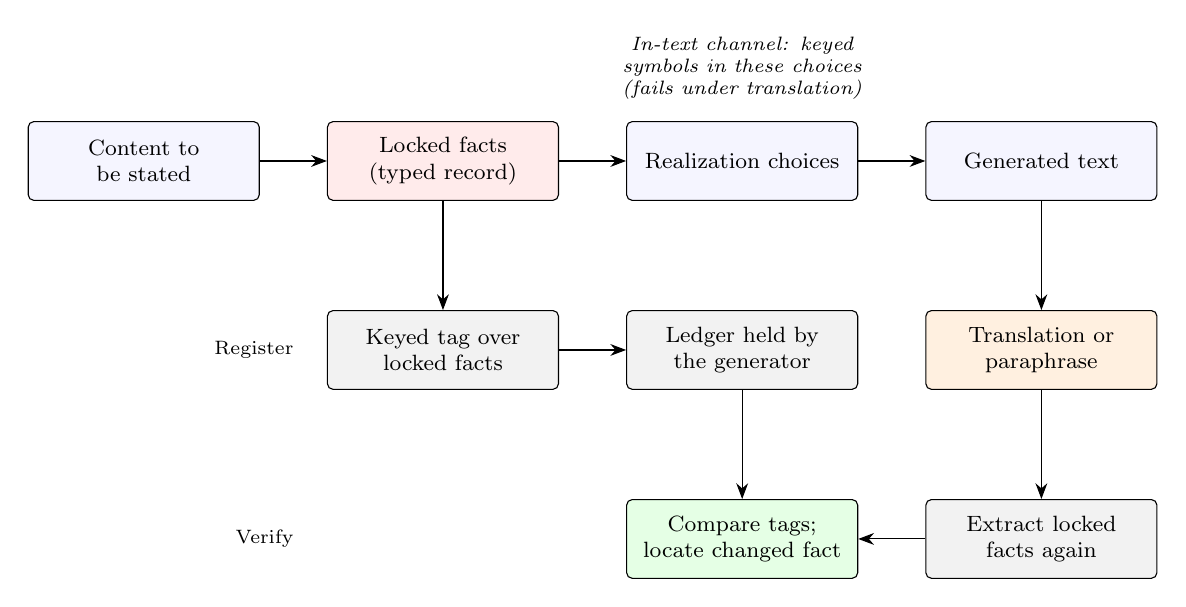
\begin{tikzpicture}[
  font=\footnotesize,
  box/.style={draw, rounded corners=2pt, align=center, minimum height=10mm, text width=27mm, fill=blue!4},
  lock/.style={box, fill=red!8}, op/.style={box, fill=black!5}, good/.style={box, fill=green!10},
  >={Stealth[length=2mm]}]
% generation (top row)
\node[box]  (x)   at (0,0)      {Content to be stated};
\node[lock] (inv) at (38mm,0)   {Locked facts\\(typed record)};
\node[box]  (rea) at (76mm,0)   {Realization choices};
\node[box]  (y)   at (114mm,0)  {Generated text};
\draw[->] (x)--(inv); \draw[->] (inv)--(rea); \draw[->] (rea)--(y);
\node[font=\scriptsize\itshape, align=center, text width=40mm, above=1.5mm of rea]
  {In-text channel: keyed symbols in these choices (fails under translation)};
% registration (middle row)
\node[op]   (tag) at (38mm,-24mm)  {Keyed tag over\\locked facts};
\node[op]   (led) at (76mm,-24mm)  {Ledger held by\\the generator};
\node[op, fill=orange!12] (tr) at (114mm,-24mm) {Translation or\\paraphrase};
\draw[->] (inv)--(tag); \draw[->] (tag)--(led); \draw[->] (y)--(tr);
% verification (bottom row)
\node[good] (chk) at (76mm,-48mm)  {Compare tags;\\locate changed fact};
\node[op]   (ext) at (114mm,-48mm) {Extract locked\\facts again};
\draw[->] (tr)--(ext); \draw[->] (ext)--(chk); \draw[->] (led)--(chk);
\node[font=\scriptsize, anchor=east] at ([xshift=-3mm]tag.west) {Register};
\node[font=\scriptsize, anchor=east] at ([xshift=-41mm]chk.west) {Verify};
\end{tikzpicture}
\caption{\textbf{Truthprint separates locked facts from free realization.} A sentence is represented as a typed record of locked facts and a set of realization choices. Two provenance channels are possible. The in-text channel hides keyed symbols in the realization choices and did not survive real translation. The ledger channel registers a keyed tag over the locked facts with the generating system; after translation or paraphrase, a verifier extracts the facts again, recomputes the tag and compares it with the ledger, and a mismatch identifies the fact that changed.}
\label{fig:pipeline}
\end{figure}

\clearpage
\begin{figure}[p]
\centering
\begin{tikzpicture}
\begin{axis}[name=a, width=80mm, height=58mm, ybar, bar width=4.2pt, ymin=0, ymax=1.05,
  symbolic x coords={RT,KO,HI,ZH,AR,DE}, xtick=data, ylabel={Documents identified},
  legend style={font=\scriptsize, at={(0.5,1.03)}, anchor=south, legend columns=3, draw=none},
  tick label style={font=\scriptsize}, label style={font=\footnotesize},
  title={\textbf{a}}, title style={at={(-0.14,1.0)}, anchor=south west}]
\addplot[fill=green!45!black] table[x=cond,y=core6] {generated/fig2a.dat};
\addplot[fill=green!25] table[x=cond,y=full9] {generated/fig2a.dat};
\addplot[fill=gray!60] table[x=cond,y=kgw] {generated/fig2a.dat};
\legend{Six-field contract, Nine-field contract, Token watermark}
\end{axis}
\begin{axis}[at={(a.east)}, anchor=west, xshift=16mm, width=80mm, height=58mm, ybar, bar width=4.2pt,
  ymin=0, ymax=1.05, symbolic x coords={RT,KO,HI,ZH,AR,DE}, xtick=data,
  ylabel={Rate}, legend style={font=\scriptsize, at={(0.5,1.03)}, anchor=south, legend columns=1, draw=none},
  tick label style={font=\scriptsize}, label style={font=\footnotesize},
  title={\textbf{b}}, title style={at={(-0.14,1.0)}, anchor=south west}]
\addplot[fill=orange!70] table[x=cond,y=sent_core6] {generated/fig2b.dat};
\addplot[fill=orange!30] table[x=cond,y=sent_full9] {generated/fig2b.dat};
\legend{{Sentence matches a wrong entry, six fields},{Same, nine fields}}
\node[font=\scriptsize, align=center, fill=white, inner sep=1pt] at (axis description cs:0.5,0.93)
  {Documents falsely attributed: 0 in every condition};
\end{axis}
\end{tikzpicture}
\caption{\textbf{Provenance of meaning survives real machine translation.} \textbf{a}, Fraction of documents identified after translation of the 50-document corpus into Korean (KO), Hindi (HI), Chinese (ZH), Arabic (AR) and German (DE) and through Korean back into English (RT), for the six- and nine-field contracts, and for a token-level watermark at a 1\% false-positive rate. The token watermark was measured on different source texts and shows signal removal, not a controlled comparison. \textbf{b}, Verification without a document identifier against a ledger of 50 documents (800 sentences): fraction of translated sentences that match at least one wrong ledger entry, and fraction of translated documents attributed to at least one wrong document (zero in every condition). $n=800$ sentences or 50 documents per condition.}
\label{fig:results}
\end{figure}

%=========================== Methods ===========================
\clearpage
%%METHODS%%
\section*{Methods}

\paragraph{Corpus and translation.} The main corpus contains 50 documents of 16 English sentences (800 sentences) generated from typed records in a closed domain of software incidents: four agents, four patients, one predicate (``fix''; ``break'' is used only as a tamper value) and two to four values each for polarity, quantity, time direction, modality, attribution and causation. Each sentence was translated with NLLB-200-distilled-600M\cite{nllb2024} into Korean, Hindi, Chinese, Arabic and German, and from English to Korean and back to English, giving 4,800 outputs. The surface-carrier pilot used four further documents translated into Korean and Hindi and back (192 outputs). A pilot for neural extraction used 16 sentences (10 templated and 6 with open wording) in six conditions (source, round trip, Korean, Arabic, Hindi and Chinese) translated by an instruction-tuned language model whose identity is not recorded in the released records; extraction used a different model from translation. No personal data and no human participants were involved.

\paragraph{Invariant extraction.} The surface (stage-1) parser reads the realization carriers of the in-text channel and is defined only for the canonical English templates. The meaning (stage-2) extractor is a hand-built six-language lexicon that maps a sentence to the nine fields after canonical normalization of numbers, entity names and time expressions. Neural extractors are instruction-tuned language models prompted with the schema and called through an OpenAI-compatible interface; their outputs are cached and released, so every reported number can be recomputed without network access.

\paragraph{Contracts, tags and the ledger.} A contract is an ordered subset of fields. Its digest is SHA-256 over the canonical JSON serialization of the contract fields. The tag is HMAC-SHA256\cite{krawczyk1997hmac} over the digest, the nonce and the sentence identifier, truncated to $\tau=32$ bits. The generator stores tags; the verifier extracts the fields from the observed text, recomputes the tag for the candidate identifier and compares in constant time. A document is attributed when at least half of its sentences authenticate. Tamper rejection registers a tag on a copy of the source record in which one contract field is set to a different valid value and tests whether the extracted record from the unaltered translation fails against it. The false-positive rate tests a translated sentence against the tag of a randomly chosen different sentence.

\paragraph{Verification without an identifier.} The verifier receives a translated document and searches all 50 registered documents. A translated sentence matches a registered document if it authenticates against any of that document's 16 sentences, because the verifier does not know the alignment. A document is attributed to every registered document matched by at least half of its sentences. We report the fraction of translated sentences that match at least one sentence of another document, the fraction of documents attributed to their own source, and the number of false attributions over all 49 other documents for each of the 50 translated documents (2,450 pairs per condition).

\paragraph{Collision floor.} The false-positive floor of a contract is the probability that two independently drawn records coincide, $\sum_v p_v^2$ over record values $v$, estimated from the empirical distribution of records in the corpus; its negative logarithm is the collision entropy. For identifier-free document attribution under independence, a translated sentence matches a 16-sentence document with probability $q=1-(1-p)^{16}$ and a document pair is falsely attributed with probability $\Pr[\mathrm{Bin}(16,q)\ge 8]$.

\paragraph{In-text channel.} The authenticated payload is the message concatenated with a tag over the message, nonce and invariant digest; it is protected by a systematic binary linear code and mapped onto realization carriers through a keyed permutation that depends on the invariant record, so that no global rule such as ``passive means one'' exists. Carriers whose candidates fail validation are recorded as erasures. Detection inverts the keyed map and decodes with erasures, and attributes only if the tag verifies. Capacity and the minimum reliable length follow from treating each carrier as a symbol on an erasure channel.

\paragraph{Baselines.} The token-level watermark followed green--red list sampling\cite{kirchenbauer2023kgw} with $\gamma=0.25$ and $\delta=2.0$ on GPT-2 generations, translated with the same NLLB system and detected with a $z$-test calibrated to a 1\% false-positive rate; these detector scores were computed on a GPU notebook that is released, but the raw scores are not yet in the repository. For the matched comparison every method scored documents of 16 sentences sampled from the 800 sentences (300 documents per condition); positive documents verify each translation against its own source, null documents against a different sentence, and each method's threshold was set at a 1\% false-positive rate on its null documents. The SemStamp-style detector\cite{hou2024semstamp} partitions a static multilingual sentence embedding (potion-multilingual-128M) with four keyed hyperplanes and is granted ideal generation, that is each source sentence is assumed to lie in its keyed region; it is our re-implementation, not the authors' system. SimHash\cite{charikar2002simhash} uses 64 keyed hyperplanes with a Hamming tolerance of 19; MinHash\cite{broder1997minhash} uses character shingles with a similarity threshold of 0.5. The retrieval baselines store each source sentence and accept a candidate whose similarity to its own source exceeds a threshold calibrated for benign acceptance of 0.95, optionally followed by a directional token-coverage entailment check or by an oracle that knows the correct record.

\paragraph{Paraphrase and adaptive attacks.} Benign operators (voice alternation, time-phrase reordering, verb and time synonyms within the lexicon, and a discourse hedge) were applied to 200 documents of 16 sentences. The adaptive attacker replaces the predicate and time expressions with synonyms outside the closed lexicon; the held-out attack uses synonyms outside the extended lexicon as well. A removal is counted as valid only if verification fails and the meaning, judged against the generating record, is unchanged.

\paragraph{Formal properties.} (i) If the validator accepts a candidate only when its extracted record equals the intended one, every emitted sentence preserves its locked facts. (ii) An adversary that causes authentication of a record never tagged by the generator yields an existential forgery against the truncated MAC. (iii) If the truncated MAC behaves as a pseudorandom function, an independently produced candidate passes a 32-bit tag check with probability $2^{-32}$, and $Q$ tested key--nonce pairs give the union bound $Q\,2^{-32}$. These bounds apply to a candidate that reaches tag verification; parsing, search, replay and the contract-collision floor determine system-level error. The 20,000-trial check of (iii) is reproduced by the released self-test.

\paragraph{Statistics.} Rates are reported with Wilson 95\% score intervals\cite{wilson1927}. All sampling uses fixed seeds, recorded with each result file.

\paragraph{Use of AI tools.} AI coding and writing assistants were used to write software, analysis scripts and drafts of the text. The author designed the study, checked every reported number against the released result files and is responsible for the content.

\paragraph{Data availability.} The source records, all 4,800 translations, the cached neural extractions and every result file are available in the public repository \url{https://github.com/leemgs/truthprint} (directory \texttt{paper/results}).

\paragraph{Code availability.} All code, including the extractors, the provenance scheme, every evaluation script and the scripts that generate the tables and figures of this paper, is available at \url{https://github.com/leemgs/truthprint} under the MIT licence. Except for the token-watermark baseline, every result can be recomputed on a CPU.

% no references first cited here


\paragraph{Acknowledgements.} None.

\paragraph{Author contributions.} G.L. conceived the study, designed and implemented the system, performed the experiments and wrote the paper.

\paragraph{Competing interests.} The author declares no competing interests.

\paragraph{Additional information.} Correspondence and requests for materials should be addressed to Geunsik Lim (leemgs@gmail.com).

%=========================== Extended Data ===========================
\edtable{1}{Recovery of each field after real translation}{ed_stage2}
\par\smallskip{\singlespacing\footnotesize\noindent Fraction of sentences whose field matches the source record after translation, stage-2 lexicon extractor, 800 sentences per condition. Abbreviations as in Table 1.\par}

\edtable{2}{Authentication by contract and condition}{ed_provenance}
\par\smallskip{\singlespacing\footnotesize\noindent core6: polarity, quantity, time, attribution, predicate, agent. robust7: core6 plus modality. full9: all nine fields. Document attributed when at least half of its 16 sentences authenticate (Wilson 95\% interval); identifier-addressed verification; 800 sentences and 50 documents per condition.\par}

\edtable{3}{Verification without a document identifier}{ed_ledger}
\par\smallskip{\singlespacing\footnotesize\noindent Ledger of 50 documents (800 sentences). False document attributions counted over all 49 other documents for each of 50 translated documents.\par}

\edtable{4}{False-positive floor set by contract collisions}{ed_collision}
\par\smallskip{\singlespacing\footnotesize\noindent Probability that two records drawn from the corpus distribution coincide, compared with the $2^{-32}\approx2.3\times10^{-10}$ bound of the tag.\par}

\edtable{5}{Matched comparison on language-model translations}{ed_matched16}
\par\smallskip{\singlespacing\footnotesize\noindent Same protocol as Table 1 on 16 base sentences translated by a language model (no German condition); the 300 documents per condition resample these 16 sentences.\par}

\edtable{6}{Ledger retrieval and entailment baselines}{ed_retrieval}
\par\smallskip{\singlespacing\footnotesize\noindent Closed-domain English paraphrases, 960 sentences; benign acceptance calibrated near 0.95; identifier-addressed.\par}

\edtable{7}{Rule-based paraphrase operators}{ed_paraphrase}
\par\smallskip{\singlespacing\footnotesize\noindent Six-field contract, closed lexicon, 200 documents of 16 sentences. Valid removal: verification fails while meaning is preserved.\par}

\edtable{8}{Neural and lexicon extractors on a small pilot}{ed_neural}
\par\smallskip{\singlespacing\footnotesize\noindent 16 base sentences in six conditions (96 records), of which 6 base sentences have open wording.\par}

\edtable{9}{Detection of single-field tampering in the closed domain}{ed_challenge}
\par\smallskip{\singlespacing\footnotesize\noindent 300 documents of 24 sentences; fraction of single-field meaning-altering edits detected.\par}

\end{document}
